%\documentclass[a4paper]{article}
\documentclass[11pt]{article}
\usepackage[T1]{fontenc} 
\usepackage[utf8]{inputenc}	%Needed if you use pdflatex instead of xelatex
\usepackage[english]{babel}
%%\pdfminorversion=4 

%\setlength{\headheight}{16pt}
%\usepackage[dvips]{graphicx} 
\usepackage{graphicx,psfrag,epsf}
%\usepackage{tikz} %Import DIA-graphs
\usepackage{amssymb,amsmath,bm}	%'gather' environment
\usepackage{flexisym}
\usepackage{xcolor,lipsum}
\usepackage{breqn}	%Use the dmath-environment to break math eq. automatically!
\usepackage{booktabs,fixltx2e}
\usepackage{setspace}
\usepackage{threeparttable}
\usepackage{epstopdf}
\usepackage{pdflscape}	%Allow landscape style pages
%\usepackage{subfig}
\usepackage{subfigure}
\usepackage{longtable}
\usepackage{fancyvrb}
\usepackage{url}
\usepackage{hyperref}
%\usepackage{float}		% for making text float around figures
\usepackage{enumerate}
%\usepackage{verbatim}
%\usepackage{framed}		%frame around text
%\usepackage[capposition=top]{floatrow}	%Add notes to figures
%\usepackage{multicol}
\usepackage{supertabular}
%\usepackage{floatrow}	%includes the \floatfoot command for notes for figures
\usepackage{todonotes}
\usepackage{makecell}	% add line break within table; https://tex.stackexchange.com/questions/2441/how-to-add-a-forced-line-break-inside-a-table-cell

% CAPTION settings
%\usepackage{caption}
%\captionsetup{font=small,labelfont=sc,textfont=it,format=plain,justification=centering,labelsep=newline,tablename=TABLE}
%\captionsetup[figure]{labelfont=normal, justification=raggedleft, labelsep=period,textfont=small}
%\floatsetup[table]{capposition=top} %style=plain


\definecolor{darkblue}{rgb}{0.055,0.094,0.588}
\definecolor{darkred}{rgb}{0.4,0,0.0157}
\definecolor{myblue}{rgb}{0.2,0.2,0.7}
\definecolor{myred}{rgb}{0.9,0,0}
\newcommand{\jemph}[1]{{\color{myblue}#1}}
\newcommand{\remph}[1]{{\color{myred}#1}}
\newcommand{\subsize}[1]{\footnotesize{#1}}	%gretl tables

\usepackage{hyperref}
\usepackage{natbib}


%\pdfminorversion=4
% NOTE: To produce blinded version, replace "0" with "1" below.
\newcommand{\blind}{0}

% DON'T change margins - should be 1 inch all around.
\addtolength{\oddsidemargin}{-.5in}%
\addtolength{\evensidemargin}{-.5in}%
\addtolength{\textwidth}{1in}%
\addtolength{\textheight}{1.3in}%
\addtolength{\topmargin}{-.8in}%


\begin{document}

%\bibliographystyle{natbib}

\def\spacingset#1{\renewcommand{\baselinestretch}%
	{#1}\small\normalsize} \spacingset{1}


%%%%%%%%%%%%%%%%%%%%%%%%%%%%%%%%%%%%%%%%%%%%%%%%%%%%%%%%%%%%%%%%%%%%%%%%%%%%%%

\if0\blind
{
	\title{\bf Practical Empirical Research Using Gretl and Hansl}
	%\title{\bf Improved Monetary Forecasts by Means of Economic Uncertainty Measures and Regularisation Techniques}
	\author{Artur Tarassow\thanks{
			The author is grateful to XXX for helpful comments. Any remaining errors or omissions are strictly our own.}\hspace{.2cm}\\
		Department of Socioeconomics, University of Hamburg}
	\maketitle
} \fi

\if1\blind
{
	\bigskip
	\bigskip
	\bigskip
	\begin{center}
		{\LARGE\bf Practical Empirical Research Using Gretl and Hansl}
	\end{center}
	\medskip
} \fi

\bigskip
\begin{abstract}
	This article provides an introduction to the free open-source statistics and econometrics software named Gretl for cross-sectional, time-series as well as panel data. Gretl is an attempt to bridge the different demands for teaching at different levels but also by providing functionalities required for professional work. We provide basic information on Gretl and its powerful and intuitive scripting language "Hansl". We introduce Gretl and Hansl by going step-by-step from the scratch through a real-life data analysis example. Finally, we estimate a vector autoregressive dynamic regression model using Gretl for conducting impulse-response analysis as well as for forecasting purposes.
\end{abstract}

%\noindent%
%{\it Keywords:} XXX, XXX\\
%{\it JEL:} XXX; XXX

\vfill

\newpage
%\spacingset{1.45} % DON'T change the spacing!
\doublespacing

\newpage
\section{Introduction}
\label{sec:intro}
Data analysis is a vital part of the economic training and of an professional economist's daily life. Economists are trained to be sophisticated users of data, and econometrics --- the interplay of economic theory, statistics and mathematics --- is a subject which usually economics students have to attend. %A typical economics degree program comprises subjects on data management, statistics, model simulation and estimation.
Undergraduates studying economics are typically exposed courses in statistics and econometrics, covering the practice and interpretation of least-squares regression, data management and data visualisation. Graduate students learn the advanced treatments of the subject, likely involving Maximum Likelihood estimation, simulation and so on. Professional economists --- whether in public or private institutions --- are likely to find themselves using, or possibly developing, econometric methods.

Gretl is an open-source and freely available statistics and econometrics software attempting to bridge the different demands for teaching at different levels as well as professional work. It comprises a full-featured graphical interface but also a powerful scripting language called hansl. Gretl's scripting language can be seen as a domain-specific language for statistics and econometrics. Gretl handles datasets --- a matrix but with a richer structure including some meta-information %information on the data type, eventual calendar date and recorded data frequency 
--- similar to Eviews but can also deal with pure matrices and arrays such as Matlab, Gauss and Julia for advanced programming purposes.

In the following, we will introduce Gretl --- and to some extend hansl --- alongside a practical empirical example using time-series data. Nevertheless, it should be mentioned that Gretl can also deal with methods and estimators for cross-sectional as well as panel data structures.

The paper is structured as follows. The next section discusses the market of econometrics software and introduces Gretl and its scripting language hansl. Section 3 introduces Gretl's graphical user interface and explains how to conduct data basic management and analyses steps accompanied by an overview about essential commands. In Section 4 a vector autoregressive time-series model will be estimated and it will be shown how the model's dynamics can be analysed for structural or forecasting purposes. Section 5 introduces the work with matrices before Section 6 summarises.


\section{Econometric Software and Gretl}

\subsection{The 'Market' of econometrics software}
The demands placed on an econometric software are a delicate issue. For teaching purpose it makes sense to have undergraduate students work with reasonably user-friendly software --- in the easiest case controlling the software by a graphical user interface through point-and-click using the mouse. However, it makes little sense to introduce a software to undergraduates which does not support more advanced methods and does not offer a fully-fledged scripting and programming environment --- aspects which are required for an advanced treatment in graduate classes and for professionals. And of course there's a premium on teaching "marketable skills" rather than dead-end expertise.

Gretl is a program which attempts to bridge these different demands. It comprises a full-featured graphical interface (the GUI): its underlying
functionality can be driven either Gretl's scripting language or by the apparatus of menus, dialog boxes and so on. The developers try to ensure that almost everything that can be done via scripting can also be done via the GUI, and vice versa, with only few exceptions \citep{Cottrell2017}.

Gretl's main competitors are the major proprietary econometrics packages, Stata and Eviews, and also the major open-source statistical software project, R. As in Gretl, datasets and series are also basic in Stata and Eviews, and econometric functionality is supported by a wide range of built-in commands. Even though both Stata and Eviews support scripting, their respective languages are quite odd from the point of view of a programmer used to general-purpose scripting languages or Matlab-like interfaces for matrix manipulation. %\remph{One cannot define a function as such in either Stata or Eviews.}
Gretl offers the common apparatus of fully-fledged programming languages (function-calling, function-definition, declaration of and assignment to named variables of various types) similar of what is known from Matlab, R and Python.

\subsection{Gretl and Hansl}
Gretl is acronym for \textbf{G}nu \textbf{R}egression, \textbf{E}conometrics and \textbf{T}ime-series \textbf{L}ibrary. The software is available for Windows, Mac OS X as well as Linux through the official Gretl homepage: \url{http://gretl.sourceforge.net/}. It is free, open-source software which may be redistributed and/or modified under the terms of the GNU General Public License as published by the Free Software Foundation.

Gretl comprises %a large shared library,
a common command line (CLI) program and a GUI client, and makes use of reliable free and open-source software packages in the 'background' for computations, e.g. (multi-threaded) LAPACK/BLAS, fftw, GTK, gnuplot, etc. The first Gretl version was released in January 2000 and has been under active development %, mainly using the C programming language, 
since then. Its user interface is available in 17 languages thanks to an active community. Gretl is shipped with a User Guide of already 380+ pages, a Command Reference of 210+ pages, and a "A Hansl Primer" tutorial to Gretl's scripting language.%named "hansl" among additional useful documents.

%Apart from the GUI, functions can also be driven by scripting using Gretl's scripting language \textit{hansl}.
As the unique selling point, Gretl offers a high-level matrix oriented language with a syntax similar to Matlab or Gauss, and an intuitive high-level scripting language called \textit{Hansl} that is attuned to econometrics. This makes Gretl especially interesting for lecturing statistics and econometrics but also for serious research.

Hansl --- “\textbf{H}ansl’s \textbf{A} \textbf{N}eat \textbf{S}cripting \textbf{L}anguage” --- was developed over time and has become a very advanced high-level scripting language with more than 140 commands specifically tailored to the domain of econometrics to date. 
The lead developers, Allin Cottrell and Riccardo "Jack" Lucchetti, have pushed the progress of Gretl mainly through Hansl in recent times. Users and developers are asked to program and publish user-contributed function packages by means of Hansl rather than the low-level language C. A great plus of Hansl-based function packages is that it comes with a handy optional GUI integration making it possible for developers to add access to specific functions through the GUI rather than solely through functions. % Most important: Hansl is a very clean and intuitive scripting language with a very nice syntax as you will see below.
For more technical details on Hansl see \citet{Cottrell2017}.


To date Gretl \textit{natively} implements a variety of models, methods and functions among others such as: 
\begin{enumerate}
	\item Time series data: ARIMA, GARCH-type, (S)VARs and (S)VECMs, unit root and cointegration tests, State Space modelling, Kalman filter, Structural Time Series Models, mixed time-series frequencies (MIDAS), etc.
	\item Limited dependent variables: Logit, Probit, Tobit, interval regression, models for count and duration data, etc.
	\item Panel-data: Instrumental variables, Probit,
	GMM-based dynamic panel models, etc.
	\item Output models as RTF or LaTeX files, in tabular or equation format.
	\item Using gnuplot for compiling high-quality graphs.
	\item Estimation of models that are not natively present in Gretl neither handled by function packages, via the \texttt{mle} or \texttt{gmm} command block.  
	\item Support for machine learning via the LIBSVM library.
\end{enumerate}
Besides Gretl's core functionality, several addons \\ (\url{http://gretl.sourceforge.net/addons-data/addons.xml}) and numerous contributed function packages (\url{http://ricardo.ecn.wfu.edu/gretl/cgi-bin/gretldata.cgi?opt=SHOW_FUNCS}) are hosted online and are easily accessible through Gretl.

Additionally, and this may make Gretl very attractive for advanced applications, is the fact that that using Hansl one can estimate models that are not natively present in libgretl neither handled by function packages, via the \texttt{mle} command for Maximum likelihood estimation, the \texttt{gmm} command for General Methods of Moments estimation and other similar ones that require non-linear optimization. The Gretl team has implemented very efficient optimisation techniques much on the same level as what you get in Python, R or Matlab. For details and examples, we refer to Ch. 23 and 24 in the Gretl manual.

Another feature is that Gretl supports the capability to communicate with other software packages such as Stata, Python, R, Julia, Ox and Octave. See Section \ref{sec:foreign} in the Appendix for details.%The \textit{foreign}-block is an interface to include statements of other languages into a hansl script allowing to send and receive information (in the form of matrices). Thus, users can call and execute functions available in other software packages which are, for instance, currently not available in Gretl. For details see the Appendix \ref{sec:foreign}.


\section{Getting Started in Gretl}
\subsection{Gretl's Graphical User Interface}
%There are several ways to work in Gretl. 
For starters, the most intuitive way is to use the program through its built-in graphical user interface (GUI). The GUI is shown in Figure \ref{fig:GUI} and consists in total of four separate windows. At the top of the main window (see Figure \ref{fig:gui_main}) you find the menu bar comprising commands to import and manipulate data, analyse data, and manage output. Below the menu bar, the user finds information on the loaded dataset and the working directory. Most space is given to the variables list where each variable is associated with a unique ID number, the variable's name and an optional descriptive label. Below the variables list, information on the loaded dataset is given such as the total number of observations or the number (and eventual time-span) of the currently selected sub-sample, respectively. The toolbar, containing a number of useful utilities, can be found at the bottom of the window. 

The console window, as depicted in Figure \ref{fig:gui_cli}, accepts Gretl commands which can be directly executed pressing "Enter". The output will immediately appear in the console. From the command prompt, '?', you can type in commands from the Gretl language or calculate something. Try for instance,
\begin{verbatim}
? eval sqrt(25)/5
\end{verbatim}
where the \texttt{eval} command evaluates an expression and prints its value.

The icon view window (see Figure \ref{fig:gui_icon}) comprises the access to different objects such as scalar values, matrices and model objects among others --- more on this below. Lastly, the script editor, as depicted in Figure \ref{fig:gui_editor}, collects several lines of programming code into a file which can be executed all at once in a script. Serious and reproducible research relies on such scripts for recording each step of the data analysis including comments on the code.


\begin{figure}[h!]
	\centering
	\subfigure[Main Window]{\label{fig:gui_main}
		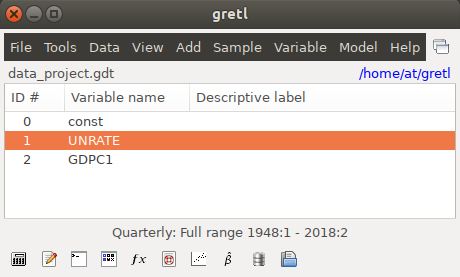
\includegraphics[width=0.44\textwidth]{../figures/gui_main}}
	%\hspace{.1in}	
	\subfigure[Console Window]{\label{fig:gui_cli}
		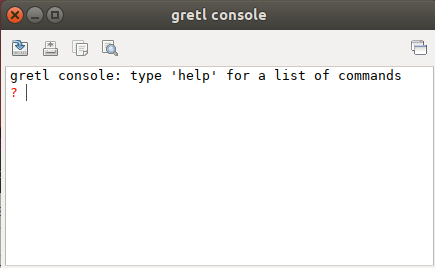
\includegraphics[width=0.43\textwidth]{../figures/gui_cli}}
	
	\subfigure[Icon View Window]{\label{fig:gui_icon}
		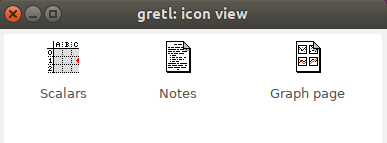
\includegraphics[width=0.44\textwidth]{../figures/gui_icon}}
	%\hspace{.1in}	
	\subfigure[Script Editor Window]{\label{fig:gui_editor}
		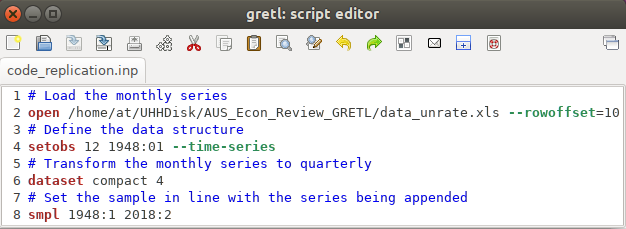
\includegraphics[width=0.44\textwidth]{../figures/gui_editor}}
	
	\caption{The Gretl Interface}
	\label{fig:GUI}
\end{figure}


Lee Adkin's (\citeyear{Adkins2014}) terrific and freely available econometrics Ebook using Gretl for the applications provides a much deeper introduction, and is highly recommended for learning and mastering Gretl (4th edition downloadable here: \\ \url{www.learneconometrics.com/gretl/using_gretl_for_POE4.pdf}; the 5th edition will be published online very soon!). Also the manual, which can be opened from the "Help, User's guide" menu, is the first source you should check in case of questions or problems.



\subsection{Loading and Appending Data}
\label{sec:dataloadappend}
Practical empirical research starts with basic data management. Gretl can import data from a variety of formats from the local hard-disk and from the internet. In the GUI program this can be done via the "File, Open Data, User file" menu. In script mode, simply use the \texttt{open} command. The supported import formats include (i) plain text files (typically comma-separated or "CSV"), (ii) spreadsheet formats as MS Excel, Gnumeric and Open Document, (iii) Stata data files (.dta), (iv) SPSS data files (.sav) and (v) Eviews workfiles (.wf1) among some others.

The following conditions must be satisfied to make sure Gretl reads data successfully:
\begin{enumerate}
	\item The first row must contain valid variable names, otherwise the program will automatically add names, v1, v2 and so on.
	\item Data values should constitute a rectangular block, with one variable per column (and one observation per row).
	\item Numeric data are expected, but in	the case of importing from plain text, the program offers handling of character (string) data.
	\item Optionally, the first column may contain strings such as	dates, or labels for cross-sectional observations
\end{enumerate}

One can append additional data either by the \texttt{append} command or via the "File, Append data" menu: Gretl will check the
new data for conformability with the existing dataset and, if everything seems OK, will merge the data. For more complex tasks, there exists the powerful \texttt{join} command (execute \texttt{help join} in the console for details).

Once data is read-in, it may be necessary to supply some information on the type of the dataset. The three types that can be distinguished are cross-section, time-series and panel data. The primary tool for doing this is the "Data, Dataset structure" menu entry in the GUI, or the \texttt{setobs} command when using scripts or the console.

In our real-world example, we deal with two macroeconomic time-series downloaded from the St, Louis Federal Reserve Bank database called FRED. % (\url{https://fred.stlouisfed.org/}).
The first series is real GDP of the U.S. economy for which data values are collected at a quarterly frequency since 1948 (\url{https://fred.stlouisfed.org/series/GDPC}). The second series refers to the civilian unemployment rate observed at monthly frequency since 1948 (\url{https://fred.stlouisfed.org/series/UNRATE}).

The two separate spreadsheets look as depicted in Figure \ref{fig:spread} with basic information on data characteristics reported in Table \ref{tab:datainfo}. The two files are stored online to allow the replication of the following example.

\begin{figure}[!h]
	\centering
	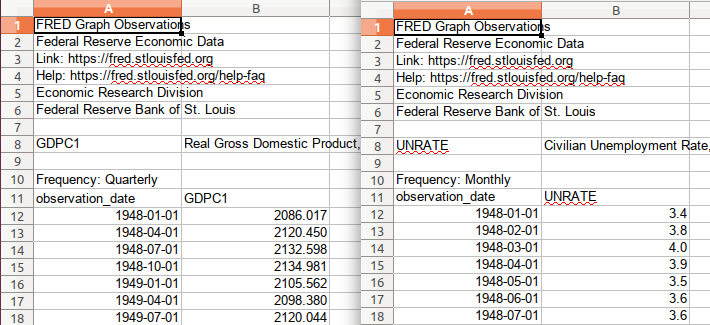
\includegraphics[width=.6\textwidth]{../figures/data_spreadsheet}
	\caption{Raw Data of Real GDP and Unemployment Rate for the U.S., Spreadsheet}
	\label{fig:spread}
\end{figure}


\begin{table}[!h]
	\centering
	\footnotesize
	\begin{tabular}{cccc}
		\hline
		Series & Frequency & Starting Date & Ending Date \\ 
		\hline 
		GDPC1	& quarterly & 1948Q1 & 2018Q2 \\ 
		UNRATE	& monthly & 1948M1 & 2018M7 \\ 
		\hline 
	\end{tabular}
	\caption{Data Information of Raw Data}
	\label{tab:datainfo}
\end{table}

Working with these two series involves at least two problems. First, the frequency among the variables differs which requires some method to equalize it. %Second, the starting date of the series is different and also needs being adjusted. Third,
Second, both series are stored in separate Excel files and need being joined. Both tasks can easily be solved.

Before proceeding, you should download both Excel-files and save them in a folder. The two xls-files can be downloaded from:
\begin{itemize}
	\item data\_unrate.xls: \url{https://scm.darnold.org/atecon/gretl_aer/raw/master/data_unrate.xls}
	\item data\_gdp.xls: \url{https://scm.darnold.org/atecon/gretl_aer/raw/master/data_gdp.xls}
\end{itemize}

First, we load the monthly UNRATE series stored in the "data\_unrate.xls" file via the "File, Open data, User file" menu which opens the "spreadsheed import" window (see Figure \ref{fig:load}). As the name of the first variable ('observation\_date') has its entry in the spreadsheet in column A and row 11, we start the data import of the rectangular block at this position as depicted in Figure \ref{fig:load}.

\begin{figure}[!h]
	\centering
	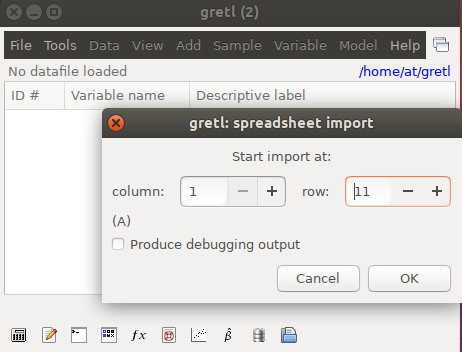
\includegraphics[width=.42\textwidth]{../figures/open_file}
	\caption{Spreadsheet Import Window}
	\label{fig:load}
\end{figure}

In case Gretl has not successfully recognized the time-series structure given some observation column (here 'observation\_date'), the user can manually determine the frequency and starting date by the menus automatically showing up in the process. Alternatively, we can set the data structure by the following command through the console
\begin{verbatim}
setobs 12 1948:1 --time-series
\end{verbatim}
where '12' refers to the number of observations per year ('12' for monthly data) followed by the initial observation date and an option saying that the data has a time series structure. The variables which appear in the main window are of the so called 'series' type.

As real GDP is only quarterly observed, we need to transform the monthly UNRATE series to quarterly observations. A standard way to do this is to compute the average of three consecutive months of a specific quarter. This is easily done via the "Data, Compact data" menu or the command
\begin{verbatim}
dataset compact 4
\end{verbatim}
which reduces the dataset from monthly to quarterly frequency. The resulting quarterly time-series will ranges 1948Q1 to 2018Q2 as indicated at the bottom of the main window.

The next step involves appending the quarterly real GDP series from another source to the existing dataset. However, when using the \texttt{append} command, we need to make sure that the currently active dataset covers the same time span as the one wished to append (the \texttt{join} command is much more flexible with regard to this). Thus, to avoid an error, we restrict the currently selected sample for the period between 1948Q1 to 2018Q2 by the command
\begin{verbatim}
smpl 1948:1 2018:2
\end{verbatim}
or through "Sample, Set range" menu using the GUI.

Appending a file can be done by using the "File, Append data" menu followed by the same request of the 'spreadsheet import' window as already shown in Figure \ref{fig:load}. Gretl automatically recognizes that the appended dataset has the same length as the active one and will add the real GDP series to the dataset. This will finally result in Figure \ref{fig:append}.

\begin{figure}[!h]
	\centering
	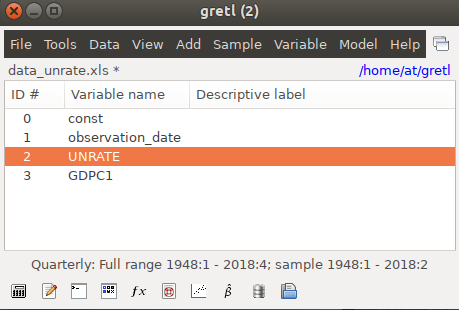
\includegraphics[width=.42\textwidth]{../figures/gretl_after_appending}
	\caption{Joint Time-Series Dataset}
	\label{fig:append}
\end{figure}

Instead of using the GUI, all previous steps from (down-)loading the data, frequency reduction and appending can be done using a collection of Gretl commands as shown in the Appendix \ref{sec:datapre}.

It should be mentioned that Gretl includes many example datasets, some of them taken from popular econometrics textbooks, which is especially useful for teaching purposes. These can be accessed through the "File, Open data, Sample file" menus. Additionally, users can easily download data from some large databases such as DB.NOMICS, quandl.com and yahoo.com:
\begin{itemize}
	\item DB.NOMICS: \url{https://next.nomics.world/}
	\begin{itemize}
		\item Access through the "File, Databases, DB.NOMICS" menu
		\item See video tutorial on youtube: \url{https://youtu.be/B2KmX9A6ICg}
	\end{itemize}
	\item Quandl: \url{quandl.com}
	\begin{itemize}
		\item Access through the \texttt{getQuandl} package: \url{http://ricardo.ecn.wfu.edu/gretl/cgi-bin/current_fnfiles/getQuandl.gfn}		
	\end{itemize}
	\item Yahoo: \url{yahoo.com}
	\begin{itemize}
		\item Access through the \texttt{yahoo\_get} package: \url{http://ricardo.ecn.wfu.edu/gretl/cgi-bin/current_fnfiles/yahoo_get.gfn}
	\end{itemize}
\end{itemize}

%Additionally, since the latest stable Gretl version (2018b) available, users can easily download data from the DB.NOMICS database (\url{https://next.nomics.world/}). See for a \textit{how-to} the following video on youtube: \url{https://youtu.be/B2KmX9A6ICg}. Also there exist user-written packages for downloading data from the \url{quandl.com} (see the \texttt{getQuandl} package: \url{http://ricardo.ecn.wfu.edu/gretl/cgi-bin/current_fnfiles/getQuandl.gfn}), and \url{yahoo.com} (see the \texttt{yahoo\_get} package: \url{http://ricardo.ecn.wfu.edu/gretl/cgi-bin/current_fnfiles/yahoo_get.gfn}) databases.


\subsection{Basic Commands}
The purpose of this section is to introduce some basic commands which are frequently executed when doing data analysis. In the following, we proceed with the dataset compiled in the previous step. Once the data is loaded, one should check its validity. %For printing data values, one can use the \texttt{print} command. However,
Initially, we will generate a so called list which can (and should!) be used to make command scripts less verbose and repetitious, and more easily modifiable. In the following, a list named \texttt{L} comprises both variables of interest namely \texttt{UNRATE} and \texttt{GDPC1}. The list is set up by the \texttt{list} command:
\begin{Verbatim}[baselinestretch=0.75, fontsize=\small]
list L = UNRATE GDPC1
\end{Verbatim}

For printing the values for each variable in a list by their respective observations, we use the \texttt{print} command with the \texttt{---byobs} option:
\begin{Verbatim}[baselinestretch=0.75, fontsize=\small]
print L --byobs
\end{Verbatim}
The corresponding output for the first five observations looks like:
\begin{Verbatim}[baselinestretch=0.75, fontsize=\small]
             UNRATE        GDPC1

1948:1      3.73333      2086.02
1948:2      3.66667      2120.45
1948:3      3.76667      2132.60
1948:4      3.83333      2134.98
1949:1      4.66667      2105.56
\end{Verbatim}

One can easily compute basic descriptive statistics for elements in a list by means of the \texttt{summary} (execute \texttt{help summary} in the console for obtaining additional options) command:
\begin{Verbatim}[baselinestretch=0.75, fontsize=\small]
summary L
\end{Verbatim}
which returns various statistics as well as information on eventual missing values:
\begin{Verbatim}[baselinestretch=0.75, fontsize=\small]
                   Mean           Median        Minimum        Maximum
UNRATE             5.7771         5.5667         2.5667         10.667
GDPC1              8557.0         7013.6         2086.0          18507

                   Std. Dev.     C.V.          Skewness   Ex. kurtosis
UNRATE             1.6318        0.28245        0.62860       0.096705
GDPC1              4956.1        0.57919        0.44045        -1.1495

                   5% perc.      95% perc.       IQ range   Missing obs.
UNRATE             3.5050         9.0617         2.2083              0
GDPC1              2465.1          17234         9046.0              0
\end{Verbatim}

In case one wants to compute these descriptive statistics using only observations for a specific sub-set, say between 1980Q1 and 2007Q4, one simply needs to restrict the sample accordingly before calling the summary command:
\begin{Verbatim}[baselinestretch=0.75, fontsize=\small]
smpl 1980:1 2007:4
summary L
\end{Verbatim}

One can also restrict the underlying sample in a more complicated way. For instance, running the command 
\begin{Verbatim}[baselinestretch=0.75, fontsize=\small]
smpl UNRATE>4 && UNRATE <= 9.6 --restrict --replace
\end{Verbatim}
would restrict the selected dataset to observations which fulfil the criteria that \texttt{UNRATE} is greater 4 but equal or less than 9.6, and replace any eventual previous restrictions imposed by the \texttt{---replace} option. %\footnote{An overview about logical operators can be found in Table \ref{tab:logic} in the Appendix.}
The user will be informed that the currently selected sample includes only 237 out of all 282 valid observations, as depicted in Figure \ref{fig:smpl}. The information that the restricted sample is "undated" states that due to the restrictions imposed, the time-series structure of consecutive observations has been broken. The original full sample with a time-series structure can be restored by the
\begin{Verbatim}[baselinestretch=0.75, fontsize=\small]
smpl full
\end{Verbatim}
command.


\begin{figure}[!h]
	\centering
	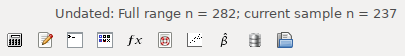
\includegraphics[width=.42\textwidth]{../figures/smpl_restrict}
	\caption{Sample Selection Information After Imposed Restriction}
	\label{fig:smpl}
\end{figure}

Sometimes one wants to manipulate data entries due to wrong or missing values recorded. Let us assume that variable \texttt{UNRATE} includes a missing value for observation 1981Q2 but you know that the U.S. unemployment rate has been 7.4 \% for this observation. Replacing a valid value or a missing value for a specific observation can be simply done by the command
\begin{Verbatim}[baselinestretch=0.75, fontsize=\small]
UNRATE[1981:2] = 7.4
\end{Verbatim}
where \texttt{[1981:2]} refers to a specific index (row) identified by a date-string of variable \texttt{UNRATE}.

A basic statistics for a bivariate analysis is the correlation coefficient. The correlation coefficient can be easily computed for all pairs of variables in a list by means of the command
\begin{Verbatim}[baselinestretch=0.75, fontsize=\small]
corr L
\end{Verbatim}
which computes Pearson's product-moment correlation. Other types of correlation %such as Spearman's rho (using the option \texttt{---spearman}) and Kendall's tau (using \texttt{---kendall})
are also available --- just execute \texttt{help corr} in the console for details. The correlation between $UNRATE_t$ and $GDPC1_t$ --- where subscript $ t $ refers to the $ t $-th observation for $ t=1,\ldots, T $ --- is close to zero and is not significantly different from zero in this example:
\begin{Verbatim}[baselinestretch=0.75, fontsize=\small]
corr(UNRATE, GDPC1) = -0.01416004
Under the null hypothesis of no correlation:
t(280) = -0.236967, with two-tailed p-value 0.8129
\end{Verbatim}

An overview about some of the available descriptive statistics are listed in Table \ref{tab:descriptive}.

\begin{table}[!h]
	\centering
	\footnotesize
	\begin{tabular}{ll}
		\hline
		Command & Description \\ 
		\hline 
		\texttt{min} & Prints the minimum of the series \\
		\texttt{max} & Prints the maximum of the series \\
		\texttt{mean} & Prints the mean of the series \\
		\texttt{median(X)} & Prints the median of the series X \\
		\texttt{summary} & Prints summary statistics of the series \\
		\texttt{xtab} & Displays a contingency table or cross-tabulation for series\\ 
		\texttt{freq} & Prints/ Plots the frequency distribution of the series \\
		\texttt{corr} & Prints the pairwise correlation coefficients for series\\
		\texttt{xcorrgm} & Prints and graphs the cross-correlogram between two series \\
		\texttt{pergm} & Computes and displays the spectrum of the series \\
		\hline 
	\end{tabular}
	\caption{Examples of Descriptive Statistics in Gretl}
	\label{tab:descriptive}
\end{table}

\subsection{Plotting}
Visualising data marks an important step in empirical work. Gretl generates graphs by means of the reliable open-source tool gnuplot which is available for many platforms. Gnuplot is a very full-featured graphing program with myriad options (for details see Ch. 6 in the gretl manual). Gretl gives you direct access, via a graphical interface, to a subset of gnuplot’s options and it tries to choose sensible values for you; it also allows you to take complete control over graph details if you wish.

In a time-series context, an obvious informative graph is the time-series plot which depicts data over time. This is easily done in Gretl by (the backslash allows for line breaks)
\begin{Verbatim}[baselinestretch=0.75, fontsize=\small]
gnuplot L --with-lines=GDPC1 --with-impulses=UNRATE \
--time-series --output=display
\end{Verbatim}
and the graph can be seen in Figure \ref{fig:TSplot}. We ask \texttt{gnuplot} to plot the variables in list \texttt{L} over time using the \texttt{---time-series} option. Furthermore, we want series GDPC1 being drawn as a line but UNRATE as impulses in this example. The option \texttt{---output=display} returns immediately a plot onto the screen.

Also scatter-plots serve as standard tools for visualising relationships between variables. A simple scatter-plot between the two series included in list \texttt{L} --- augmented by a linear OLS-based regression fit --- is called by (see Figure \ref{fig:XYplot}):
\begin{Verbatim}[baselinestretch=0.75, fontsize=\small]
gnuplot L --fit=linear --output=display
\end{Verbatim}
The option \texttt{---output=filename} allows the user to specify a particular output format. Supported output formats are \textit{.eps} (Encapsulated PostScript), \textit{.pdf} (PDF) and \textit{.png} (PNG) among others. For instance, for storing a figure in png-format in a specific directory, use the expression: \\
\texttt{---output="C:\textbackslash{Project}\textbackslash{Figures}\textbackslash{Fig1}.png"}

\begin{figure}[h!]
	\centering
	\subfigure[Time-Series Plot]{\label{fig:TSplot}
		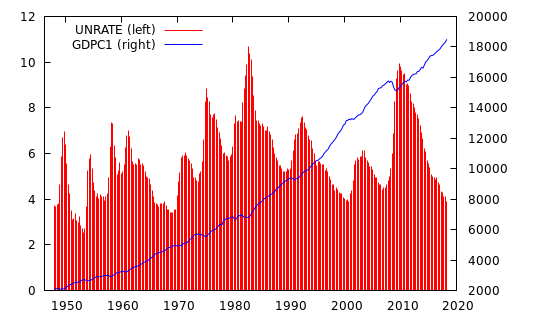
\includegraphics[width=0.44\textwidth]{../figures/TSplot}}
	%\hspace{.1in}	
	\subfigure[Scatter-Plot]{\label{fig:XYplot}
		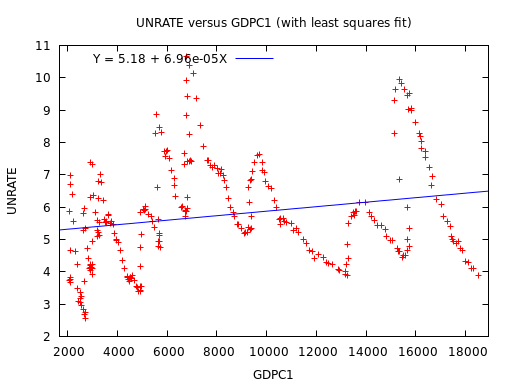
\includegraphics[width=0.44\textwidth]{../figures/XYplot}}

	\caption{Time-Series and Scatter-Plot using Gretl}
	\label{fig:Plot1}
\end{figure}

Another useful type of graph is the Boxplot which summarizes a number of descriptive statistics for the researcher. The \texttt{boxplot} command produces this type of graph. Before showing an example, however, let us generate a new series named \texttt{GreatModeration} which shall be a binary dummy variable taking the value of one for observations between 1985Q1 and 2007Q4, and otherwise zero:
\begin{Verbatim}[baselinestretch=0.75, fontsize=\small]
series GreatModeration = (obs>="1985:1" && obs<="2007:4")
print GreatModeration --byobs
\end{Verbatim}
The ones indicate the well-known Great Moderation period during which business cycle indicators such as GDP growth and price inflation rates followed a rather stable path associated with only small variance around some mean value.

Let us draw the boxplot for the \texttt{UNRATE} series and examine its distribution conditional on the value of the dummy variable \texttt{GreatModeration} by using the \texttt{---factorized} option: 
\begin{Verbatim}[baselinestretch=0.75, fontsize=\small]
boxplot UNRATE GreatModeration --factorized --output=display \
{ set title 'Distribution of UNRATE outside and during Great Moderation' ; }
\end{Verbatim}
Figure \ref{fig:Plot2} shows that the variance of the unemployment rate has indeed been smaller during the Great Moderation phase in the U.S. compared to the remaining period; even though mean and median values have been of comparable magnitude. Note that we added a self-explanatory title to the graph.

\begin{figure}[h!]
	\centering
	\subfigure[Boxplot]{\label{fig:BOXplot}
		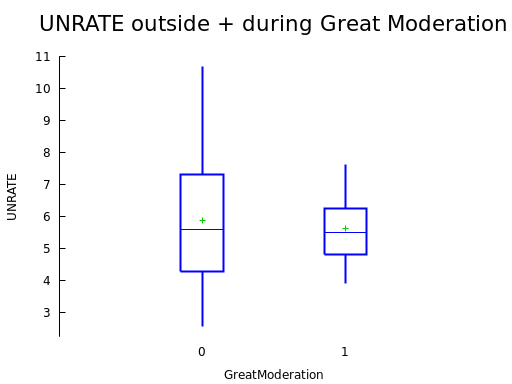
\includegraphics[width=0.44\textwidth]{../figures/BOXplot}}
	\caption{Factorized Boxplot using Gretl}
	\label{fig:Plot2}
\end{figure}



\section{Let's estimate a dynamic time-series model}
In this section we want to illustrate how to estimate a dynamic time-series model using Gretl. We will to examine the dynamic relationship between the change in the unemployment rate and growth in aggregate output (as proxied by the Gross Domestic Product). The famous macroeconomist Arthur Melvin Okun formulated a negative relationship between these two variables which has become known as 'Okun's Law'.

%\subsection{Generate variables}
Before estimating the regression model, we need to generate the two variables of interest. The following lines generate two new series objects where \texttt{dU} refers to the period-change in the unemployment rate, $ dU_t = UNRATE_t - UNRATE_{t-1} $, and \texttt{gY} refers to the (exact) period-growth rate of real GDP (in percent), $ gY_t =  100 \times \left( \frac{GDPC_t - GDPC_{t-1}}{GDPC_{t-1}}\right) = 100 \times \left( \frac{GDPC_t}{GDPC_{t-1}}-1 \right)$:
\begin{Verbatim}[baselinestretch=0.75, fontsize=\small]
series dU = UNRATE - UNRATE(-1)
series gY = 100 * (GDPC1/GDPC1(-1) - 1)
\end{Verbatim}
As can be seen, in a time-series (but also panel) context, Gretl easily handles lags and leads by using an expression such as \texttt{x(p)} where $ p $ generates the $ p $-th lag of series \texttt{x} if $p$  takes a negative and the $ p $-th lead if it takes a positive integer value.

\subsection{The VAR model}
The vector autoregressive model of order $ p $ (VAR(p)) is a commonly-used tool in macroeconomics. In its most basic incarnation it is written as
\begin{equation}
\label{eq:VAR}
	z_t = \mu + \sum_{i=1}^p \Phi_i z_{t-i} + \varepsilon_t
\end{equation}
where $z_t$ is an $k \times 1$-dimensional vector of observable quantities at time $t$, and $ \mu $ is a $k \times 1$-dimensional vector of constants. The autoregressive coefficient matrices, $\Phi_i$, are of size $ k\times k $. In our case, we set $z_t=\left[dU_t, gY_t\right]^\prime$. %The $\mu$ vector and the $\Phi_i$ matrices are unknown and must be estimated from the data.
$\varepsilon_t$ is an $k$-dimensional vector white noise process with time-invariant, positive definite covariance matrix $ E(\varepsilon_t \varepsilon^\prime_t)=\Sigma_\varepsilon $. The econometrician's job is to estimate the unknown quantities $\mu$, $\Phi_i$ and $ \Sigma_\varepsilon $ from the data so that the model can be used for policy analysis and forecasting.


%For illustration, we estimate the following linear autoregressive distributed lag (ARDL(p,q)) model
%\begin{equation}
%	\label{eq:ardl}
%	dU_t = \beta_0 + \sum_{i=1}^{p} \beta_i dU_{t-i} + \sum_{j=0}^{q} \theta_j gY_{t-j} + u_t\; , t=1, \ldots, T
%\end{equation}
%where $ dU_t $ is a function of its own $ p $ lagged values, and the contemporary as well as lagged values up to order $ q $ of growth of output, $ gY_t $. Scalar $ \beta_0 $ refers to the intercept, and the error-term $ u_t $ follows a white-noise zero mean process with constant variance $ u_t \sim WN(u, \sigma^2_u) $.
%
%The objective is to estimate the unknown parameters $ \beta $, $ \theta $ and $ \sigma^2_u $. Assuming, that $ gY_t $ is indeed exogenous w.r.t. $ dU_t $ meaning that $ gY_t $ 'causes' contemporaneously $ dU_t $ but not \textit{vice versa}, we can estimate (under stationarity of both series) eq. (\ref{eq:ardl}) by OLS.

For simplicity, we will base the estimation on a specific sub-sample ranging from 1985Q1 to 2007Q4 comprising in total $ T=92 $ valid observations as this sample is associated with parameter stability. As a consequence of two oil crises in the mid and late 1970s as well as the recent Great Financial Crisis, Okun's Law has been associated with changed model coefficients and heteroskedasticity --- so called structural breaks which violate some of the standard Gauss Markov assumptions required for an unbiased and efficient OLS estimator. The sample restriction is imposed by:
\begin{Verbatim}[baselinestretch=0.75, fontsize=\small]
smpl 1985:1 2007:4
\end{Verbatim}

\subsection{Determination of the optimal lag-order}
%We restrict the lag-orders $ p $ and $ q $ to be equal --- which of course doesn't actually have to be but simplifies things.
The unknown optimal finite lag-order $ p $ is determined by means of information criteria (see every good introductory textbook on time-series analysis for details). We use Gretl's built-in \texttt{var} command with the option \texttt{---lagselect} to determine the optimal lag order by setting the maximum lag order to test twice the data frequency (=8 for quarterly data). Gretl will estimate model eq. (\ref{eq:VAR}) (the intercept is automatically added) for eight different lag lengths and compute three standard information criteria for each lag-order. Of course, the user could also use the GUI through the "Model, Time series, Multivariate, VAR lag selection" menu for this.

Again we make use of lists, here named \texttt{ylist}, comprising both variables of interest. The commands and the corresponding output are:
\begin{Verbatim}[baselinestretch=0.75, fontsize=\small]
list ylist = dU gY
var 8 ylist --lagselect

lags    loglik    p(LR)       AIC          BIC          HQC

1      -7.70739             0.297987     0.462451*    0.364366 
2      -0.56199  0.00642    0.229608*    0.503716     0.340241*
3       1.35475  0.42901    0.274897     0.658647     0.429782 
4       3.11277  0.47544    0.323635     0.817029     0.522773 
5       4.19395  0.70592    0.387088     0.990124     0.630479 
6       6.09821  0.43254    0.432648     1.145327     0.720291 
7       8.02423  0.42640    0.477734     1.300056     0.809630 
8      14.89473  0.00817    0.415332     1.347297     0.791481 
\end{Verbatim}
While the Akaike (AIC) and Hannan–Quinn (HQC) information criteria select the optimal lag-order to be $ p^\ast = 2 $ --- resulting in a VAR(2) model --- the Schwarz (BIC) criteria selects a parsimonious VAR(1) model. We stick to the VAR(2) in the following example but the reader is invited to re-run the analysis for a VAR(1) model.

\subsection{VAR estimation and specification testing}
Estimating the VAR(2) model by means of OLS can be done by
\begin{Verbatim}[baselinestretch=0.75, fontsize=\small]
Model <- var 2 ylist	# 'Model <-' constructs a model object
\end{Verbatim}
The \texttt{var} command is followed by the lag-order and the separate names of the endogenous variables or, as done here, a list of series. Further exogenous variables as well as deterministics like a linear trend can be added (execute \texttt{help var} in the console for details).
%The intercept is not included per default but can be added by the \texttt{const} series (the built-in identifier for a constant or y-intercept).

Note the optional expression "\texttt{Model <--}" preceding the actual \texttt{var} command. This expression generates a so called model object (here named "Model") which instantly appears in the icon view (remember Figure \ref{fig:gui_icon}). A double-click on the "Model"-icon opens the "model"-window (see Figure \ref{fig:gui_model}) where the user can proceed with the GUI for evaluating the estimation results, executing various tests, structural analyses, plot several estimation-related graphs such as residuals and fitted values and do forecasting. This underlines the nice implementation of graphical objects which is especially useful for beginners and teaching.

\begin{figure}[!h]
	\centering
	%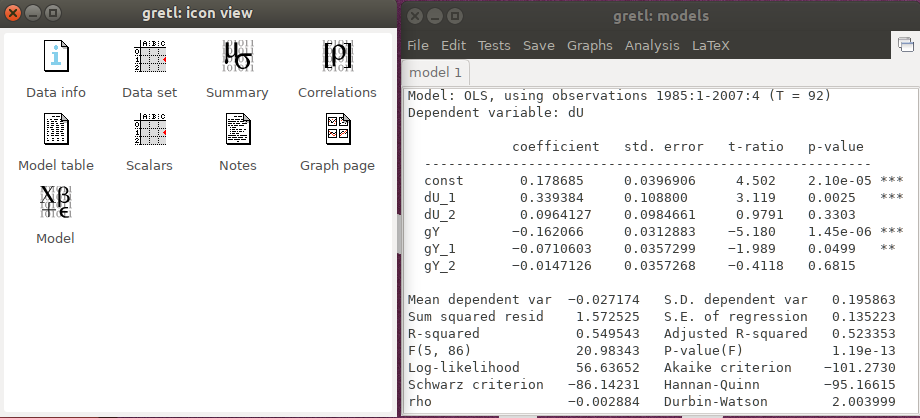
\includegraphics[width=.72\textwidth]{../figures/gui_model}
	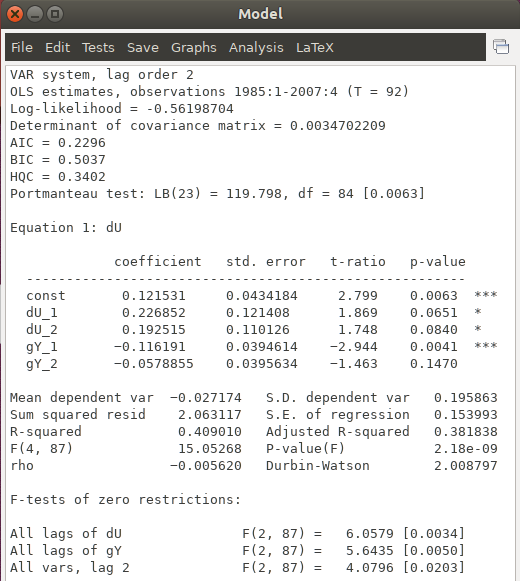
\includegraphics[width=.42\textwidth]{../figures/gui_var}
	\caption{Model Window After VAR Model Estimation}
	\label{fig:gui_model}
\end{figure}

The well-formatted estimation output covers standard estimation information for each VAR equation.
%Also note the information below the expression "F-tests of zero restrictions:" in the output. For instance, the third line in following output tests the null hypothesis that variable $ gY $ is not Granger-causing variable $ dU $. The null can be rejected at the 1\% significance level (p-value = 0.005):\todo{COuld be droppped}
%\begin{Verbatim}[baselinestretch=0.75, fontsize=\small]
%F-tests of zero restrictions:
%All lags of dU               F(2, 87) =   6.0579 [0.0034]
%All lags of gY               F(2, 87) =   5.6435 [0.0050]
%All vars, lag 2              F(2, 87) =   4.0796 [0.0203]
%\end{Verbatim}

Three diagnostic (multivariate) tests based on residuals are available after estimating a VAR model --- for normality, auto-correlation and ARCH (Autoregressive Conditional Heteroskedasticity). These are implemented by the \texttt{modtest} command, using the options \texttt{---normality}, \texttt{---autocorr} and \texttt{---arch}, respectively. For details we refer to Ch. 29.4 in the Gretl manual. The following lines illustrate the use of these commands but the tests can also be executed under the "Tests" menu in the Model Window:
\begin{Verbatim}[baselinestretch=0.75, fontsize=\small]
modtest 4 --autocorr  # test on 4th order serial correlation
modtest 4 --arch      # test for ARCH of order up to 4
modtest --normality
\end{Verbatim}

The output indicates that the model does not seem to suffer from any misspecification issues:
\begin{Verbatim}[baselinestretch=0.75, fontsize=\small]
Test for autocorrelation of order up to 4
           Rao F   Approx dist.  p-value
lag 1     0.529    F(4, 168)     0.7146
lag 2     0.457    F(8, 164)     0.8849
lag 3     0.667    F(12, 160)    0.7808
lag 4     0.803    F(16, 156)    0.6806

Test for ARCH of order up to 4
            LM       df     p-value
lag 1    10.305      9      0.3264
lag 2    16.952     18      0.5264
lag 3    24.042     27      0.6280
lag 4    27.449     36      0.8463

Doornik-Hansen test
Chi-square(4) = 4.42308 [0.3518]

\end{Verbatim}


\subsection{Structural analysis}
Gretl’s built-in \texttt{var} command supports the Cholesky decomposition-based approach, the classic and most popular "Structural VAR" (SVAR) variant. Impulse-response functions can be easily computed through the "Graphs, Impulse responses (combined)" menu in the Model Window. This opens a new window where the user can set some parameters such as the forecast horizon, the width of the confidence interval and the Cholesky ordering (see Figure \ref{fig:irfset}.
Figure \ref{fig:irfs} depicts the impulse-response results with bootstrap (per default 999 iterations) confidence intervals for each variable combination of the VAR(2) model. Computation is very fast as the underlying code is written in C. In case the user wants to use commands instead of the GUI, the steps can also be done via the command line interface by using the \texttt{---impulse-response} option when executing the \texttt{var} command.

\begin{figure}[h!]
	\centering
	\subfigure[Settings for Impulse Response Analysis]{\label{fig:irfset}
		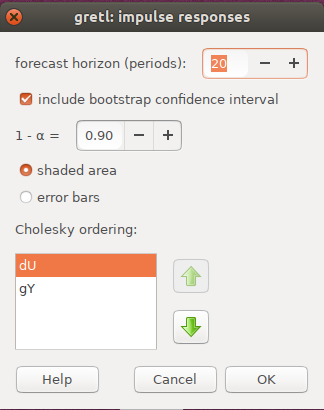
\includegraphics[width=0.3\textwidth]{../figures/gui_setirf}}
	\subfigure[Results with 90\% bootstrap confidence intervals]{\label{fig:irfs}
		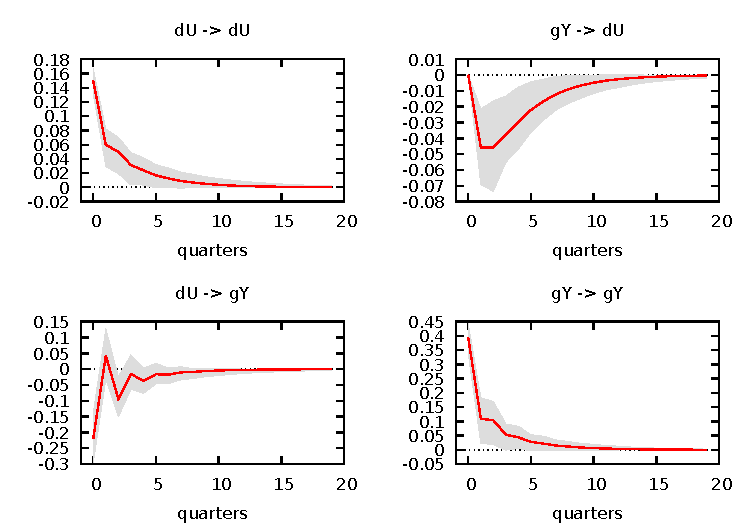
\includegraphics[width=0.6\textwidth]{../figures/irfs}}
	\caption{Impulse Response Functions with Bootstrap Confidence Intervals}
	\label{fig:IRF}
\end{figure}

Another tool, the so called Forecast Error Variance Decomposition, can be called through the Model Window through the "Graphs, Forecast variance decomposition" menu in a similar vein as done for impulse responses, or by the \texttt{---variance-decomp} option when executing the \texttt{var} command. We would also like to emphasize that the presented tools are also available for the "vector error-correction model" (VEC) model framework considering cointegration relationships between non-stationary series. Additionally, more advanced identification methods are included in the Gretl add-on \texttt{SVAR} which can be downloaded through the "Help, Check for addons" menu and which comes with a detailed manual accessible through the console by \texttt{help SVAR}. The SVAR functions can be called through the "Model, Time series, Multivariate, Structural VARs" menu.

\subsection{Out-of-sample forecasting}
Lastly, given our in-sample based estimates ending in 2007Q4, we want to forecast the dynamics of $ dU_t $ for the following quarters. This is called an out-of-sample forecasting exercise. Again, the user can use the \texttt{fcast} command for scripting or the Model Window GUI for doing this. When using the latter approach, forecast settings can be called through the "Analysis, Forecasts" menu in the Model Window. The settings for the forecast analysis are depicted in Figure \ref{fig:fcset}, and the forecasting results with 95\% intervals are shown in Figure \ref{fig:fc}. Obviously, our VAR(2) has failed to capture the rapid rise in the change in the unemployment rate as a result of the Great Financial Crisis in 2008/9. See Ch. 32.5 in the Gretl manual for details on how VAR-based forecasts are computed.

The \texttt{fcast} command also involves the option to compute basic forecast evaluation statistics, as can be seen when executing:
\begin{Verbatim}[baselinestretch=0.75, fontsize=\small]
fcast 2008:1 2018:2 --dynamic
\end{Verbatim}


\begin{figure}[h!]
	\centering
	\subfigure[Settings for Forecast Analysis]{\label{fig:fcset}
		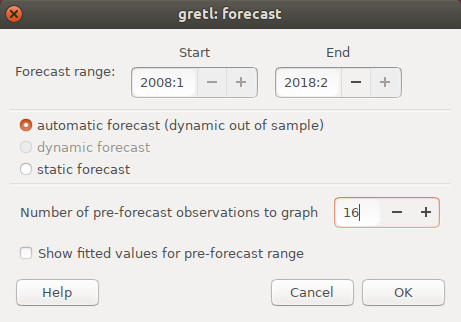
\includegraphics[width=0.41\textwidth]{../figures/gui_setfc}}
	\subfigure[Out-of-sample Forecast of $ dU_t $]{\label{fig:fc}
		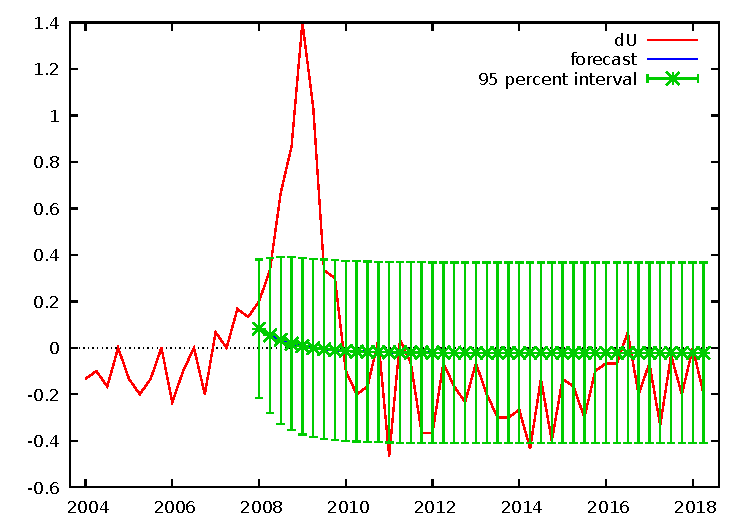
\includegraphics[width=0.44\textwidth]{../figures/fcvar}}
	\caption{VAR Forecast Analysis}
	\label{fig:FC}
\end{figure}





%Before proceeding with the model interpretation, one needs to run specification tests to check whether the Gauss-Markov criteria are fulfilled by the estimated model. Using commands instead of the GUI, the estimated residuals are depicted in Figure \ref{fig:uhat} and can be directly accessed after having executed the \texttt{ols} command by the $ \$uhat $ accessor (for a list of available accessors, click the menu "Help, function reference"):
%\begin{Verbatim}[baselinestretch=0.75, fontsize=\small]
%series resid = $uhat	# store residuals as series object
%gnuplot resid --with-lines --time-series --output=display
%\end{Verbatim}
%
%The following four lines run a battery of specification tests. The \texttt{modtest} command calls various built-in specification tests such as tests on no remaining serial correlation in the residuals of order $ k $ (using \texttt{k ---autocorr}), the White's test on homoskedasticity (\texttt{---white}) and more (see \texttt{help modtest} for details). The command \texttt{reset} calls Ramsey's RESET test on the correct functional form while \texttt{qlrtest} performs the Quandt likelihood ratio test for no structural break at an unknown point in time. Many more standard tests are easily accessible for cross-sectional, time-series and panel-data models. The \texttt{---quiet} option suppresses auxiliary regressions which may be deactivated if one wants to understand how the respective tests are actually performed.
%
%\begin{Verbatim}[baselinestretch=0.75, fontsize=\small]
%modtest 1 --autocorr --quiet	# test on 1st order serial correlation
%modtest --white --quiet
%reset --quiet
%qlrtest --plot=display
%\end{Verbatim}

%The output indicates that the model does not seem to suffer from any misspecification issues and also there is no hint on parameter breaks at any point in time (see Figure \ref{fig:qlr}):
%\begin{Verbatim}[baselinestretch=0.75, fontsize=\small]
%Breusch-Godfrey test for first-order autocorrelation
%Test statistic: LMF = 0.030358,
%with p-value = P(F(1,85) > 0.0303584) = 0.862
%
%White's test for heteroskedasticity
%Test statistic: TR^2 = 12.437424,
%with p-value = P(Chi-square(20) > 12.437424) = 0.900198
%
%RESET test for specification (squares and cubes)
%Test statistic: F = 2.831376,
%with p-value = P(F(2,84) > 2.83138) = 0.0646
%
%Quandt likelihood ratio test for structural break at an unknown point,
%with 15 percent trimming:
%The maximum F(6, 80) = 1.38908 occurs at observation 2000:3
%Asymptotic p-value = 0.870269 for chi-square(6) = 8.33445
%\end{Verbatim}
%
%\begin{figure}[h!]
%	\centering
%	\subfigure[Residuals]{\label{fig:uhat}
%		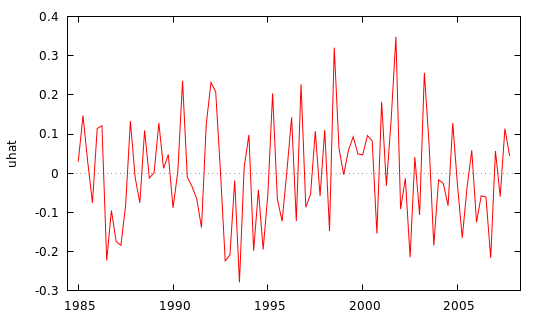
\includegraphics[width=0.44\textwidth]{../figures/uhat}}
%	\subfigure[QLR test results]{\label{fig:qlr}
%		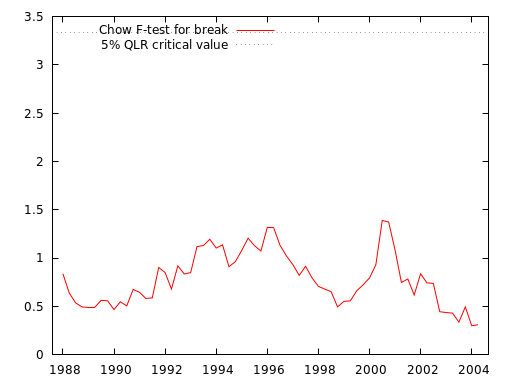
\includegraphics[width=0.44\textwidth]{../figures/QLR}}
%	\caption{Estimated residuals, $ \hat u_t $ and Quandt likelihood ratio test results on parameter stability}
%	\label{fig:QLR}
%\end{figure}

%After having checked the model's specification, we compute the dynamic multipliers using the ARDL(2,2) coefficient estimates. The so called impact multiplier refers to the immediate change in the endogenous, $ dU_t $ after a unit-change in $ gY_t $: $ \frac{\partial dU_t}{\partial gY_t} = \hat \theta_0 = -0.162$ in period $ t $. A percentage point increase in growth of real GDP leads to a reduction of the change in the unemployment rate by about 0.162 percentage points in the same quarter. The long-run multiplier, $ \hat \theta^{lr}$, is a non-linear expression computed as $ \hat \theta^{lr} = \frac{\sum_{j=0}^2 \hat \theta_j}{1-\sum_{i=1}^{2} \hat \beta_i} = -0.439$. Using Gretl we can directly compute these two multiplier values by grabbing the OLS coefficient estimates using the \texttt{\$coeff} accessor as follows:
%
%\begin{Verbatim}[baselinestretch=0.75, fontsize=\small]
%printf "Impact multiplier = %g\n", $coeff(gY)
%scalar lr_theta = ($coeff(gY)+$coeff(gY_1)+$coeff(gY_2)) / \
%(1-$coeff(dU_1)-$coeff(dU_2))
%printf "Long-run multiplier = %g\n", lr_theta
%\end{Verbatim}
%yielding the following values
%\begin{Verbatim}[baselinestretch=0.75, fontsize=\small]
%Impact multiplier = -0.162066
%Long-run multiplier = -0.439273
%\end{Verbatim}


\section{Working with matrices}
%Gretl uses the fully-fledged linear algebra library \textit{lapack}.
Gretl's matrix language has similarity to the syntax of widespread commercial software packages such as MATLAB and GAUSS. The Gretl project allows an easy transfer of series objects to the matrix-world, and \textit{vice versa}. For details on matrix manipulations, matrix algebra, statistics and transformations see Ch. 16 in the Gretl manual.

The following example shows how we could have estimated the VAR(2) model easily by means of standard linear algebra using the solution to the minimization problem underlying standard OLS. The solution is the famous equation $ \hat \beta = (X^\prime X)^{-1} X'y $ where $ y $  is a $ T \times k $ vector of the endogenous, $ [dU_t, gY_t] $, and $ X $ is the $ T \times p*k $ matrix of $ k $ regressors and $ p $ lags (disregarding the intercept vector).

We declare the two matrix objects \texttt{y} and \texttt{X} by defining the respective matrices. The $ \hat \beta $-matrix, \texttt{bhat}, is easily computed by using the \texttt{inv()} function for computing the inverse of a matrix, and \texttt{'} is a shortcut for the transpose of a matrix (equal to the \texttt{transp()} function). The commands for doing all necessary steps are:
\begin{Verbatim}[baselinestretch=0.75, fontsize=\small]
matrix y = {dU}~{gY}   # takes eventually restricted sample into account
list xlist = const dU(-1 to -2) gY(-1 to -2)
matrix X = {xlist}
bhat = inv(X'X)*X'y
bhat = bhat'		# transpose k by 2 matrix
colnames(bhat, "const dU_1 dU_2 gY_1 gY_2")
rownames(bhat, "dU-eq: gY-eq:")
printf "%12.6g\n", bhat
\end{Verbatim}
The \texttt{printf} command prints the result
\begin{Verbatim}[baselinestretch=0.75, fontsize=\small]
              const        dU_1        dU_2        gY_1        gY_2
dU-eq:     0.121531    0.226852    0.192515   -0.116191  -0.0578855
gY-eq:     0.352663     0.69436   -0.592979    0.278473     0.26639
\end{Verbatim}
which is exactly the coefficient matrix we have obtained before by the \texttt{var} command as shown in Figure \ref{fig:gui_model}.


\section{Summary}
Our intent has been to introduce the statistics and econometrics software Gretl and its scripting language Hansl. Gretl handles standard data types for doing data analysis. The language supports commands as well as a fully-fledged programming language. Commands are accessible either via a graphical user interface or a command line. The software includes many functions tailored for statistics and econometrics purposes. Additionally, Gretl's community has programmed and published over 100 additional addons or packages continuously extending its functionalities. These features declare Gretl a serious competitor on the market for statistics and econometrics software which should be considered by students, teachers as well as professionals.

This paper has provided a step-by-step guide ranging from data loading, management and initial analysis over model specification and testing up to model analysis. We have estimated a dynamic vector autoregressive time-series model and shows how easily one can conduct a structural as well as forecasting analysis using Gretl.

We want to mention that Gretl is a continuously developing software. Interested users are asked to post Gretl-related questions, to request features and to report bugs on the Gretl mailings (\url{http://gretl.sourceforge.net/lists.html}). Furthermore, everybody is encouraged to develop user-contributed packages on which an open-source statistics and econometrics software heavily relies on.


% #############################################################
% #																														#
% #					 						LITERATURE CITED											#
% #																														#
% #############################################################
%\newpage 
%%%%%%%%%%%%%%%%%%%%%%%%%%%%%%%%%%%%%%%%%%%%%%%%%%%%%%%%%%%%%%%%%%%%%%%%%
\addcontentsline{toc}{section}{REFERENCES}
\bibliographystyle{apalike} % chicago, apalike, aes

% Local folder path
\bibliography{../../../UHHDisk/05_Literatur_DATENBANK/library.bib}

\newpage

% #############################################################
% #																														#
% #					 							DATA APPENDIX												#
% #																														#
% #############################################################
\appendix
\setcounter{table}{0}
\renewcommand{\thetable}{A\arabic{table}}
\setcounter{figure}{0}
\renewcommand{\thefigure}{A\arabic{figure}}

\section{Appendix}

%\subsection{Further Resources}
%\remph{
%\begin{itemize}
%	\item youtube tutorials ???
%	\item \todo{Add link to user list for gretl-related questions and bug reports}
%\end{itemize}
%}



\subsection{Data Preparation and Cleaning Process}
\label{sec:datapre}
Below is a script for loading, defining, transforming, appending and storing the dataset used in Section \ref{sec:dataloadappend}. The script replicates all steps which were done using the GUI elements in Section \ref{sec:dataloadappend} before. Copy and paste the following commands into a new script file in the editor window (see Figure \ref{fig:gui_editor}) and execute all commands by pressing "Ctrl+R".

\begin{Verbatim}[baselinestretch=0.75, frame=single, fontsize=\small]
clear			# clear memory
set verbose off	# avoid printing commands

# Define a string variable for the URL where files are located
string url = "https://scm.darnold.org/atecon/gretl_aer/raw/master"
print url

# Load the monthly series from the server
open "@url/data_unrate.xls" --rowoffset=10 --preserve

# Define the data structure
setobs 12 1948:01 --time-series

# Transform the monthly series to quarterly
dataset compact 4

# Set the sample in line with the series being appended
smpl 1948:1 2018:2

# Append the real GDP series from the server
append "@url/data_gdp.xls" --rowoffset=10

# Drop the series 'observation_date'
delete observation_date

# Store the two time-series in native Gretl data format (*.gdt)
store "data_project.gdt"	# alternatively one can use "*.csv"
# Open the clean project file
open "data_project.gdt"
\end{Verbatim}


\subsection{Add-ons and Contributed Packages}
Both add-ons and (user-contributed) function packages add functionalities such as estimators, hypothesis tests or other analytical procedures to gretl's repertoire of built-in procedures. A list (including manuals) of available add-ons can be found here: \url{http://gretl.sourceforge.net/addons.html}. A list of contributed packages including a help test or manual and sample script can be accessed here: \url{http://ricardo.ecn.wfu.edu/gretl/cgi-bin/gretldata.cgi?opt=SHOW_FUNCS}

For details on function packages read the "Gretl Function Package Guide" which can be downloaded by clicking the "Help, Function package guide" menu.

Function packages can either be acquired through the GUI or the command line. Using the command line, one needs to download (at least once to store it on the hard-disk) the package from the package server, and load it into memory at the beginning of each gretl session. A function package ships new functions which can be called. For details one has to read the help text or manual of a specific package. The following commands illustrate the steps:
\begin{Verbatim}[baselinestretch=0.75, frame=single, fontsize=\small]
install ADMBP		# download package from server
include ADMBP.gfn	    # load into memory
help ADMBP		   # opens help text or pdf-manual (if available)
\end{Verbatim}


%\subsection{Econometric Models}
%\remph{TBW}


%\subsection{Logical Operators}
%\label{sec:logop}
%The following logical operators are supported in Gretl. 
%
%\begin{table}[!h]
%	\centering
%	\footnotesize
%	\begin{tabular}{ll}
%		\hline
%		Logical symbol & Meaning \\ 
%		\hline 
%		== & Is equal to \\
%		!= & Is not equal to \\ 
%		\&\& & And \\
%		|| & Or \\
%		> & Greater than \\
%		>= & Greater than or equal to \\
%		< & Less than \\
%		<= & Less than or equal to \\
%		\hline 
%	\end{tabular}
%	\caption{Logical Operators}
%	\label{tab:logic}
%\end{table}

%\subsection{\textit{if}-conditions}
%\remph{TBW}

\subsection{Loops}
For details read Ch. 12 in the Gretl manual. The command \texttt{loop} opens a special mode in which gretl accepts a block of commands to be repeated zero or more times. The general form of a loop is:
\begin{Verbatim}[baselinestretch=0.75, fontsize=\small]
loop control-expression [ --progressive | --verbose | --quiet ]
	loop body
endloop
\end{Verbatim}
Gretl supports various loop control variants such as "Count", "While", "Index", "Foreach" and "For" loops. 
%\begin{enumerate}
%	\item Count loop: \texttt{loop 1000} for repeating the loop 1000 times
%	\item While loop: \texttt{loop while essdiff > .00001} will continue so long as the specified condition evaluates as true
%	\item Index loop: \texttt{loop i=1..20} runs a loop from 1 to 20 which is incremented by one round
%	\item Foreach loop: \texttt{loop foreach i peach pear plum} for executing the loop once for each string in the list
%	\item For loop: \texttt{loop for (r=0.01; r<.991; r+=.01)} \texttt{r} will take on the values $ 0.01, 0.02, \ldots, 0.99 $ across the 99 iterations
%\end{enumerate}

\subsection{Functions}
For details read Ch. 13 in the Gretl manual. Gretl offers a mechanism for defining functions, which may be called via the command line, in the context of a script, or (if packaged appropriately, see section 13.5) via the program’s graphical interface. The syntax for defining a function looks like this:
\begin{Verbatim}[baselinestretch=0.75, fontsize=\small]
function type funcname (parameters)
	function body
end function
\end{Verbatim}

Here is an example for the use of functions:
\begin{Verbatim}[baselinestretch=0.75, fontsize=\small]
# function definition
function scalar ols_ess (series y, list xvars)
	ols y 0 xvars --quiet
	printf "ESS = %g\n", $ess
	return $ess
end function

# main script
open data4-1
list xlist = 2 3 4
# function call (the return value is ignored here)
ols_ess(price, xlist)
\end{Verbatim}


\subsection{Communication with other software packages}
\label{sec:foreign}
Gretl support the communication with other popular software packages. Through the so called "foreign mechanism" the user can interpolate into a hansl script a set of statements to be executed by another program, with apparatus available to ferry data between the programs. This facility is supported for Octave, R, Python, Ox, Stata and Julia. This is especially useful to exploit functionality in the "foreign" program that is not currently available in Gretl. For details see ch. 39 to 44 in the Gretl manual.


\end{document}



